% Author: Animesh Garg
% Date: June 23, 2013

\section{INTRODUCTION}
\label{sec:introduction}
% Motivate the problem

%Every year, \todo{X} cases of cancer are treated with Radiation therapy in United States.
Almost two-thirds of all cancer patients receive Radiation Therapy treatment. Over 25 million patients are treated annually with radiation therapy 
in US alone \cite{american2010physician}. External Beam Radiation Therapy, along with its variations, is a common form of radiotherapy treatment. 
With external beam radiation therapy, radiation is usually administered as a complex combination radiation beams directed at the tumor. 
Advanced techniques of dose calculation and treatment delivery are employed to 
permit design of treatment fields to maximize the differential in dose 
delivered to tumors and healthy tissue \cite{hendee2013radiation, schweikard1993motion, chui2001inverse}.

Stereotactic radiosurgery is a minimally invasive form of surgical intervention 
which makes use of a three-dimensional coordinate system to locate small 
targets inside the body and to perform a treatment operation on the targets.
A single high dose fraction of radiation is stereotactically directed to a region of interest inside the body.
 
Accuracy and precision in patient positioning is essential for success of 
external beam radiation delivery systems, particularly stereotactic radiosurgery.. Since radiation therapy is delivered over 
multiple sessions, repeatability of a patient positioning system is important 
to maintain registration between the patient and radiation delivery equipment.

Presently, a variety of standard patient positioning  systems are employed in 
clinical procedures.This leads to problems in maintaining conformance between
simulated and physically delivered radiation dose distributions over multiple 
sessions. Furthermore, these patient positioning systems are inconvenient 
for the patients often requiring local anesthesia to relieve pain.\todo{cite}

One of the most widely known stereotactic radiosurgery systems is the Gamma Knife \cite{de1989stereotactic}.A Gamma Knife typically contains 201 cobalt-60 sources which collectively aim gamma radiation onto a frame containing patient's head. Cyber-Knife is also a very popular frameless robot assited stereotactic radiosurgery method \cite{coste2005robotic}.

%Give example of the problem
For instance, stereotactic radiotherapy (SRT) is used primarily for treating 
tumors in the brain. The procedure has sub-millimeter accuracy, but assumes 
exact patient to machine registration. Commercially available head positioning 
solutions for SRT usually require the patient's head to be placed in a cubical 
frame with multiple screws securing the head in its place. One example of such
a system is illustrated in figure~\ref{fig:leskellFrame}. The screws cause discomfort and the frame only allows the head to be placed in a fixed set of orientations.

An ideal positioning system should allow a continuous change in orientation of the head. This freedom allows the physicians to plan for radiation delivery with relative ease, because some orientations would reduce volume of healthy tissue between tumor and source. 


%state our solution
%The key insight in building a principled solution for immobilization is 
%customization to patient anatomy. 
We propose a patient specific approach which uses surplus
point contacts than required for form closure and also uses surface contacts. 
This higher degree of customization is also facilitated by
recent advances in stereolithography and 3D printing.\cite{Lipson2013, gershenfeld2007fab}

A 3D-reconstruction of the patient anatomy is performed using a CT (or MRI) scan. Then, we use surplus contact points and surface contacts to the set of minimal grasp points required for immobilization (form closure). This minimizes maximum force at any contact point, thereby improving comfort The submodularity of grasp coverage allows some additional contact points while reducing the max contact force. Calculation of the subset of contact points can be performed in a reasonable time. \todo{refine}


\begin{figure}[t!]
  \begin{center}
    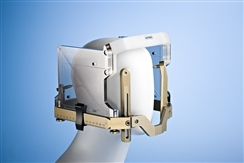
\includegraphics[width=0.8\linewidth]{images/leskellFrame}
  \end{center}
  \vspace{-10pt}
\caption{ The figure shows a Leskell Coordinate Frame-G, from Elekta, used for Stereotactic Radiosurgery.
As illustrated in the picture, the patient head is placed in a frame and secured in place with 
use of 4 screws}
  \vspace*{-15pt}
  \label{fig:leskellFrame}
\end{figure}


%list claims and their significance. (Use forward referencing instead of explicit roadmap of the paper. )
This study builds upon the previous work from Schulman et al 
\cite{schulman2011grasping}. In this paper,
\begin{itemize}
\item We describe an algorithm which minimizes maximum contact force and 
immobilizes the subject.
\item We evaluate the performance of algorithm on multiple instances of \todo{X} 
body parts.
\item We create a patient specific head positioning system using 3D printing.

\end{itemize}


